\documentclass[12pt,a4paper]{article}
\usepackage{graphicx}
\title{Team Report}

\begin{document}

\maketitle

\section{Introduction}
Before designing the project we addressed the ambiguities in the specification.
Many of these ambiguities were related to the student sign up and registration
processes.

For example, in order to register a student for the next period of study, the
teacher  should "calculate the weighted mean grade" and then "determine
whether a student may progress". The wording of these use cases certainly suggest that
these tasks would be carried out by the teacher, not our system. However, we assumed
that this was actually meant to be interpreted the other way, i.e. the system
would calculate the weights, and be able to determine the students progression
(otherwise why would the specification have given us grade boundaries and details on what
type of mean was to be be used?)

The sign up for modules was also open to interpretation. It was laid out that
Registrars were able to add and drop modules on behalf of the student, whilst
students were able to 'sign up' for a suitable number of modules. We interpreted
teh...

A third ambiguity in the specification came where it says that Administrators can
'add and remove user accounts'. It is also stated that Registrars can 'add and remove
students'. The ambiguity here lies in whether or not a student is encompassed within
the term 'user', i.e. should an Administrator be able to create students or not? We
settled on no, as during student creation we assign a degree to a student, and this
seems much more appropriate for a Registrar to do.


\section{Use Case Diagram}

% centered image for the use case diagram
\centerline{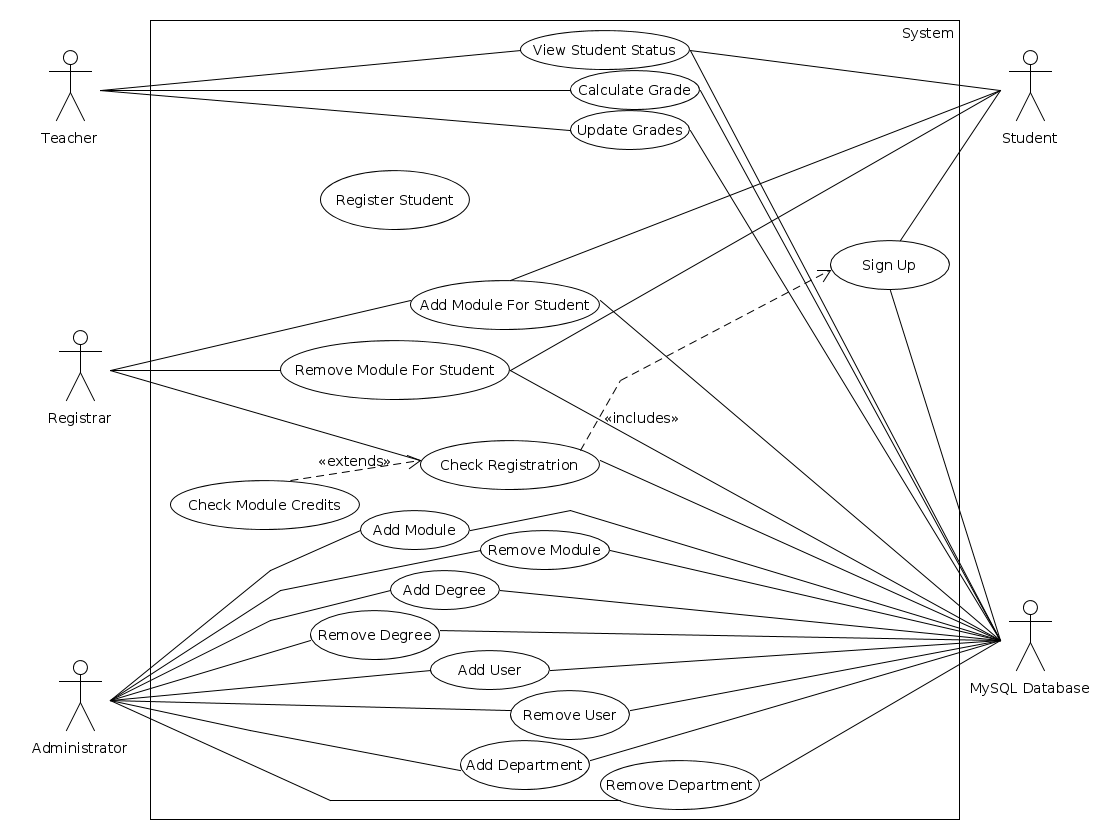
\includegraphics[width=20cm]{useCaseDiagram}}

\section{Class Diagram}

\section{Database Design}

\section{State Machine Diagram}

\section{Features of the System}

\section{Security Considerations}

\section{Conclusion}

\end{document}
